\documentclass[conference]{IEEEtran}
\IEEEoverridecommandlockouts
\usepackage{cite}
\usepackage{amsmath,amssymb,amsfonts}
\usepackage{algorithmic}
\usepackage{graphicx}
\usepackage{anyfontsize}
\usepackage{titlesec}
\usepackage{url}
\usepackage{hyperref}
\usepackage{xcolor}

\hypersetup{
    colorlinks=true,
    linkcolor=blue,
    filecolor=magenta,      
    urlcolor=cyan,
}

\begin{document}

\title{\textbf{Interpret American Sign Language}}

\author{\IEEEauthorblockN{Abrar Ahmed}
\IEEEauthorblockA{\textit{Department of Computer Science and Engineering} \\
\textit{BRAC University}\\
Dhaka, Bangladesh \\
abrar.ahmed1@g.bracu.ac.bd}
\and
\IEEEauthorblockN{Zarin Tasnim Raisa} 
\IEEEauthorblockA{\textit{Department of Computer Science and Engineering} \\
\textit{BRAC University}\\
Dhaka, Bangladesh \\
zarin.tasnim.raisa@g.bracu.ac.bd}
}

\maketitle

\begin{abstract}
  \hspace{0.5ex}
  This report focuses on developing and comparing a Convolutional Neural Network (CNN) model for interpreting American Sign Language (ASL) gestures, aiming to enhance communication for individuals with hearing and vocal impairments. We conducted preprocessing and model training, evaluating the performance of both models on a dataset of hand sign images representing ASL gestures. Our findings underscore the efficacy of CNNs for ASL gesture recognition, emphasizing the model’s potential in crafting practical sign language recognition systems to enhance accessibility and communication for individuals with disabilities.
\end{abstract}

\vspace{\baselineskip}

\begin{IEEEkeywords}
  \hspace{1ex}
  Machine Learning, Convolution Neural Network,  Long Short-Term Memory, Image Processing, Sign Language Recognition 
\end{IEEEkeywords}

\section{Introduction}

{\LARGE S}{ign} language serves as the primary mode of communication for individuals with hearing and vocal impairments, greatly impacting their daily interactions. To address the challenges faced by this demographic, we propose the development of a system aimed at facilitating communication.
\vspace{\baselineskip}

American Sign Language (ASL) involves hand shapes, movements, and facial expressions, all integral to conveying meaning. Our system focuses on recognizing static gestures of ASL, encompassing the letters a-i and k-y. We did not work with the J and Z alphabets, as we can not determine them from static images. ASL was chosen due to its widespread usage among the hearing-impaired population.
\vspace{\baselineskip}

We used LabelBinarizer to convert the 1D Labels of the images to a 1D binary array in preference to our model. We reshaped and flattened our images for the same purpose. These two features are then classified using the Convolution Neural Network (CNN), effectively mapping gestures to their corresponding alphabets.

\vspace{\baselineskip}
Our Contributions - 

\begin{itemize}
  \item We are introducing a novel system to facilitate communication for individuals with speech and vocal disabilities.
  \item We are proposing improved methods for hand sign language detection.
\end{itemize}

\vspace{\baselineskip}
\vspace{\baselineskip}
\vspace{\baselineskip}

The paper is organized as follows -

\begin{itemize}
  \item Section II reviews past Research \& our Dataset.
  \item Section III describes the Methodology.
  \item Section IV presents Experimental Results \& comparisons between other models.
  \item Section V concludes our approach to interpreting American Sign Language.
\end{itemize}

\vspace{\baselineskip}
\section{Literature Review \& Dataset}
\vspace{\baselineskip}
{\LARGE S}ome related works apply Machine Learning methods to interpret sign languages. Anup Kumar, Karun Thankachan, and Melvinevin M. Dominic [1] used Support Vector Machines, Adaboost, SVM classifiers, and Zernike Moments for Sign Language Detection in real time. Aishwarya, Aparna, and Divya Jennifer D’Souza [2] used the Convolution Neural Network model and Naive Bayes Classifier to recognize Sign Language from static images.  Ahmed, S., Kar, S. K., \& Basak, S. [3] applied Naive Bayes, Support Vector Machine, Random Forest, and K-Nearest Neighbors for Sign Language Recognition and achieved 97\% accuracy. 

\vspace{\baselineskip}

\textbf{Data Set:} The model used an image dataset from Kaggle. The dataset contains one column for Label and 784 columns for Pixels. Pixels columns are labeled from Pixel1 to Pixel784. There are 27455 rows, each representing an image. Each Pixel column contains values from 0 to 255 representing the pixel's intensity.

\begin{center}
  \makebox[0.8\linewidth]{%
      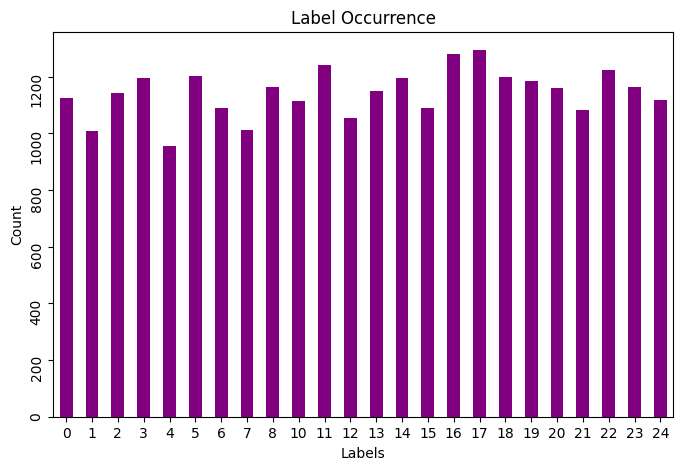
\includegraphics[width=0.9\columnwidth]{E:/Courses/CSE427/Project/Latex/DatasetLabelOccuranceGraph}
  }
  
  \textbf{Figure 1:} Occurrence of Labels in the Dataset
\end{center}

\vspace{\baselineskip}


\section{Methodology}

\vspace{\baselineskip}


\titleformat{\subsection}[runin]{\bfseries}{}{0pt}{}

\subsection{\textbf{A. Data Pre-Processing:}} 
In the realm of data analysis and machine learning, data comes in various formats, including images, audio, video, and structured tables. However, machines perceive data differently than humans. Instead of directly interpreting visual or auditory content, machines process data as binary digits - 1s and 0s.
For example, an image is seen by a machine as a grid of pixel values encoded in binary form. Similarly, audio files are translated into numerical representations of sound waves, and textual documents are converted into numerical vectors.
Therefore, leveraging machine learning to analyze diverse data forms requires preprocessing and transformation. This step involves converting raw data into structured representations that machines can process. Through techniques like image encoding, audio feature extraction, and text vectorization, raw data is translated into numerical inputs for algorithms.

\vspace{\baselineskip}

\textbf{Steps in Data Preprocessing:}

\vspace{\baselineskip}

1. Initially, we delved into the dataset's diversity by examining the labels, each representing a distinct sign language gesture. With a total of 24 unique labels, encompassing the alphabet from 'a' to 'i' and 'k' to 'y' in American Sign Language (ASL), we gained insights into the breadth of sign language representations within the dataset. In the process of preparing the data for machine learning tasks, such as classification, we needed categorical labels to be transformed into a 1D binary format for our model to process. This transformation is crucial for our classification because our model requires numerical input. One common technique for this is called one-hot encoding, where each unique label is represented as a binary vector. We used the LabelBinarizer from scikit-learn to perform one-hot encoding on the ‘label’ column in our dataset.

\vspace{\baselineskip}

2. To optimize our image data for neural network processing, we first restructured it to a more appropriate format. This involved converting each image from its original 1D vector form to a 2D array with dimensions of 28x28 pixels. By doing so, we ensured alignment with the input specifications of our model. Subsequently, we flattened these 2D arrays back into 1D vectors, streamlining their integration into our neural network architecture for seamless analysis and training. To reduce complexity and ensure fewer errors when training a model, we recommend converting it to a 2D image array and then converting it to a 1D vector format.

\subsection{B. Classifier - Convolutional Neural:}

Data classification involves organizing data into categories based on their attributes. This process helps in understanding and predicting different classes within the data. For example, it could determine whether a loan application is risky or safe. There are two main steps involved: first, learning about the data to create a classification model, and second, using that model to classify new data into the appropriate categories.

\vspace{\baselineskip}

We have utilized Convolutional Neural Network (CNN) to classify images within our dataset. CNNs are deep learning models specifically designed for image recognition tasks. The process involves several layers:

\vspace{\baselineskip}

\begin{itemize}
    \item \textbf{Convolutional Layers}: Convolutional layers are pivotal components of Convolutional Neural Networks (CNNs) employed in image processing tasks. These layers utilize learnable filters, or kernels, to perform convolution operations on input images. During convolution, filters traverse the input image, computing dot products with corresponding pixels to extract features like edges, textures, and patterns. Convolutional layers often incorporate activation functions, like ReLU, to introduce non-linearity, and parameters such as padding and stride to control output feature map dimensions.
    
    \vspace{\baselineskip}

    \begin{center}
      \makebox[1\linewidth]{%
          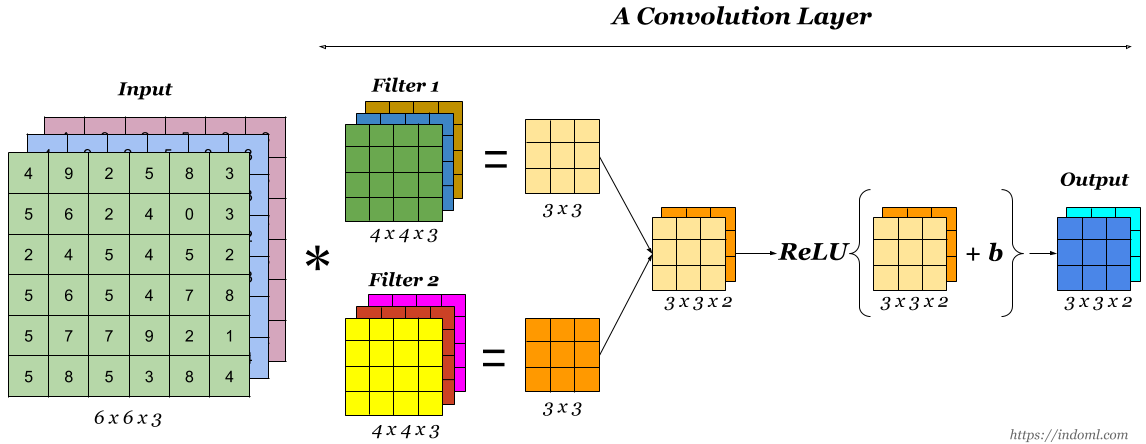
\includegraphics[width=1\columnwidth]{E:/Courses/CSE427/Project/Latex/ConvolutionLayer}
      }

      \vspace{\baselineskip}

      \textbf{Figure 2:} Convolutional Layer
    \end{center}

    \vspace{\baselineskip}

    \item \textbf{Pooling Layers}: Pooling layers, such as max pooling, are components commonly found in Convolutional Neural Networks (CNNs) used for image processing tasks. These layers serve to downsample the feature maps produced by convolutional layers, reducing their spatial dimensions while retaining important information. Max pooling, for instance, partitions the input into smaller subregions and outputs the maximum value from each subregion, effectively summarizing key features. This downsampling process helps in reducing computational complexity, alleviating overfitting, and enhancing translation invariance within the network architecture. We have used max-pooling in our model.
    
    \vspace{\baselineskip}

    \begin{center}
      \makebox[1\linewidth]{%
          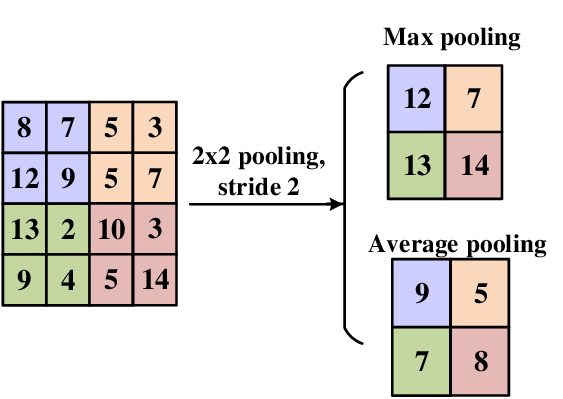
\includegraphics[width=0.5\columnwidth]{E:/Courses/CSE427/Project/Latex/PoolingLayer}
      }

      \vspace{\baselineskip}

      \textbf{Figure 3:} Pooling Layer
    \end{center}

    \vspace{\baselineskip}

    \item \textbf{Flattening}: The output from the convolutional and pooling layers is flattened into a one-dimensional vector to be fed into the fully connected layers.
    
    \vspace{\baselineskip}

    \item \textbf{Dense Layers}: These layers use the extracted features to classify images into different categories. They connect every neuron in one layer to every neuron in the next layer, enabling complex pattern recognition.
    
    \vspace{\baselineskip}

    \item \textbf{Output Layer}: The final layer produces the classification output, typically using activation functions like softmax for multi-class classification.
    
    \vspace{\baselineskip}

    \begin{center}
      \makebox[1\linewidth]{%
          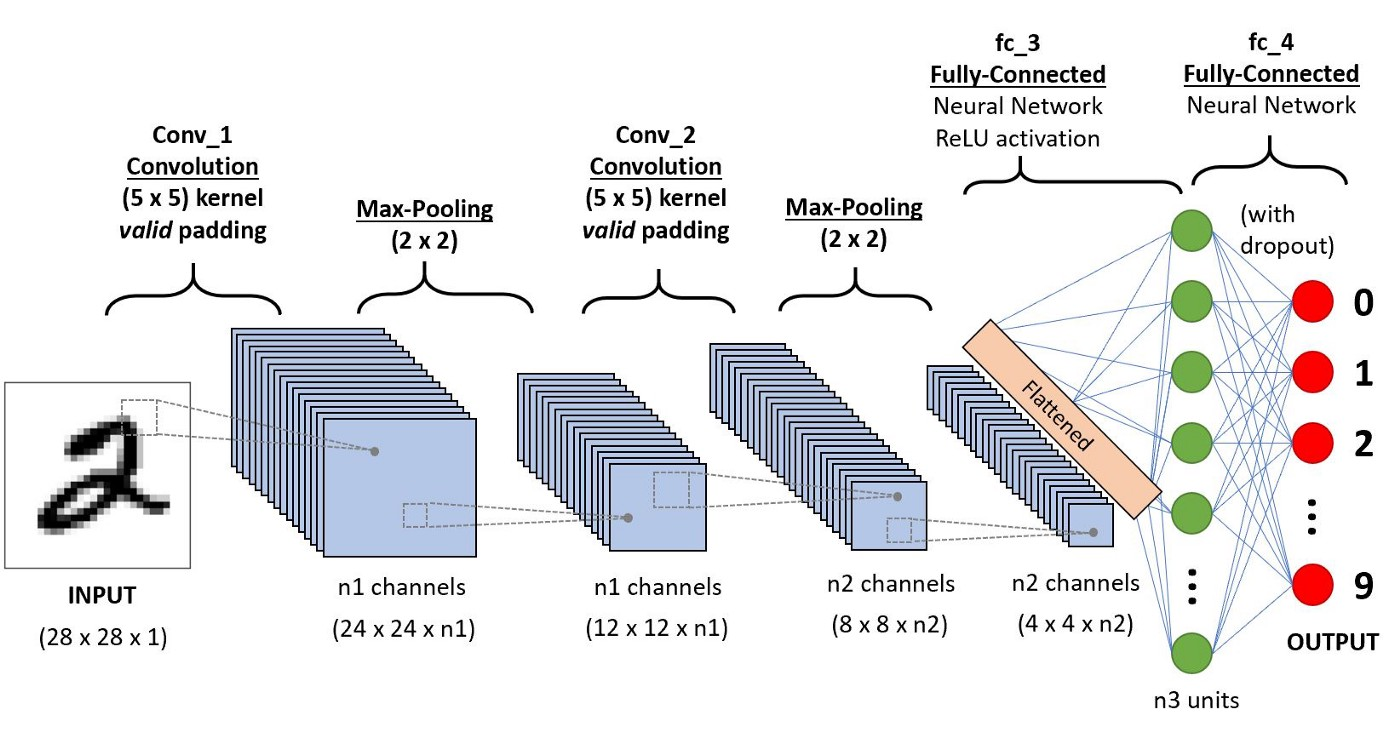
\includegraphics[width=1\columnwidth]{E:/Courses/CSE427/Project/Latex/CNN}
      }

      \vspace{\baselineskip}

      \textbf{Figure 4:} CNN Model Overview
    \end{center}

    \vspace{\baselineskip}

\end{itemize}

Our model is constructed by sequentially adding layers, each contributing to the feature extraction and classification process. We have used multiple convolution layers and max pooling layers in our model. Repeated convolutional and max pooling operations serve the crucial role of capturing progressively abstract and complex features from the dataset. Through this iterative process, the network learns hierarchical representations of the input data, facilitating effective classification and analysis.

\vspace{\baselineskip}

\subsection{C. Dataset Splitting and Fitting into CNN:}

In the dataset-splitting phase, the data was divided into training and testing sets to assess the model's performance. This process helps evaluate the model's generalization ability and prevents overfitting.
The \texttt{train\_test\_split} function from the scikit-learn library was used to split the dataset into training and testing sets. This function randomly shuffles and splits the data into two subsets based on the specified proportion, typically a percentage of the data reserved for testing.

\vspace{\baselineskip}

We split the dataset into four sets:

\vspace{\baselineskip}

\begin{itemize}
    \item \textbf{x\_train} Training data features (Images) used to train the model.
    \item \textbf{x\_test} Testing data features (Images) used to evaluate the trained model.
    \item \textbf{y\_train} Training data labels (Labels) corresponding to \texttt{x\_train}.
    \item \textbf{y\_test} Testing data labels (Labels) corresponding to \texttt{x\_test}.
\end{itemize}

\vspace{\baselineskip}

Subsequently, the \texttt{x\_train} and \texttt{y\_train} subsets were utilized to train the CNN model, while predictions were made on both \texttt{x\_test} and \texttt{y\_test} subsets to evaluate the model's performance.

\section{Experimental Result}

\vspace{\baselineskip}

We have set our model’s epoch to 10. It means the model was trained and evaluated on the dataset 10 times to iteratively improve its accuracy and performance. After training the Convolutional Neural Network (CNN) model on the sign language dataset, we obtained promising results during the evaluation phase. The model achieved an impressive accuracy of approximately 97.77\% on the testing dataset, indicating its proficiency in accurately classifying sign language gestures. These results underscore the effectiveness of the CNN architecture in learning and recognizing complex patterns within image data, demonstrating its potential for practical applications in sign language recognition systems.

\vspace{\baselineskip}

\begin{center}
  \makebox[1\linewidth]{%
      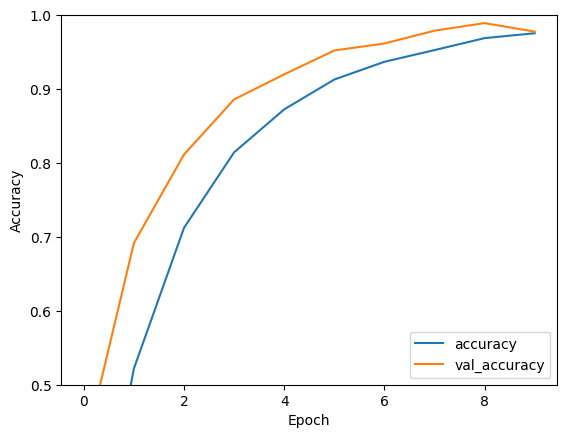
\includegraphics[width=1\columnwidth]{E:/Courses/CSE427/Project/Latex/cnnAccuracy}
  }

  \textbf{Figure 5:} CNN Accuracy Graph
\end{center}

\vspace{\baselineskip}

\section{Comparison Between Other Model}

\vspace{\baselineskip}

\subsection{Model Complexity:}

\textbf{CNN} typically have simpler architectures compared to LSTMs, consisting of convolutional and pooling layers followed by fully connected layers.
\textbf{LSTM} have more complex architectures, incorporating recurrent connections to capture temporal dependencies over time.


\subsection{Performance:}


In our experiments, the \textbf{CNN model} achieved an impressive accuracy of approximately 97.77\% on the testing dataset, demonstrating its proficiency in accurately classifying static ASL gestures.
On the other hand, the \textbf{LSTM model} achieved an accuracy of approximately 92.12\% on the testing dataset.

\vspace{\baselineskip}

\subsection{Comparison of Accuracy}

Upon evaluation, the CNN model achieved a higher accuracy of approximately 97.77\% compared to the LSTM model, which attained an accuracy of approximately 92.12\%. Therefore, it can be inferred that the CNN model outperforms the LSTM model in accurately classifying ASL gestures based on the provided dataset.

\vspace{\baselineskip}

\begin{center}
  \makebox[1\linewidth]{%
      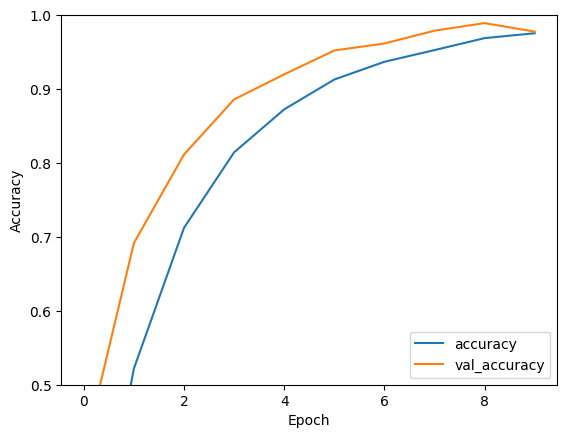
\includegraphics[width=1\columnwidth]{E:/Courses/CSE427/Project/Latex/cnnAccuracy}
  }
  \makebox[1\linewidth]{%
      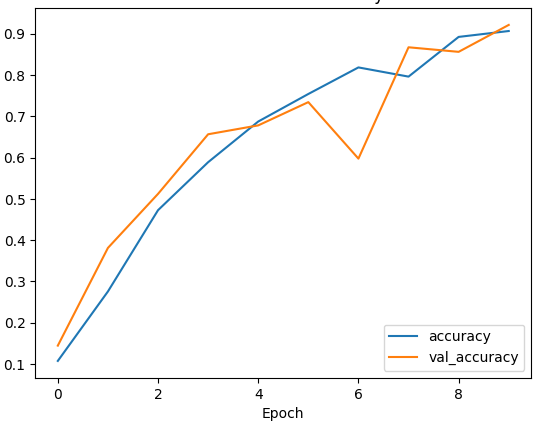
\includegraphics[width=1\columnwidth]{E:/Courses/CSE427/Project/Latex/lstmAccuracy}
  }

  \textbf{Figure 6:} Comparison Graph: CNN and LSTM's Accuracy 
\end{center}


\vspace{\baselineskip}

In summary, CNN is well-suited for recognizing static ASL gestures than LSTM.

\vspace{\baselineskip}

\section{Conclusion}

In this report, we aimed to develop the Convolutional Neural Network (CNN) for interpreting American Sign Language (ASL) gestures, with the overarching goal of facilitating communication for individuals with hearing and vocal impairments. Our initial steps involved exploring a dataset comprising hand sign images representing various ASL gestures. Through preprocessing, we reshaped and flattened the images while one-hot encoding the labels, preparing the dataset for model training.

\vspace{\baselineskip}

For the CNN model, we devised a deep learning architecture consisting of convolutional and pooling layers to extract spatial features from the images, followed by dense layers for classification. The CNN model underwent training and evaluation using a designated portion of the dataset reserved for testing.

\vspace{\baselineskip}

Upon evaluation, the CNN model exhibited superior performance, achieving a test accuracy of approximately 97.77\%. We compared the accuracy with the LSTM model's accuracy of approximately 92.12\%. This outcome underscores the efficacy of CNN in interpreting ASL gestures, attributed to its capability to recognize hand sign languages.

\vspace{\baselineskip}

In conclusion, our report underscores the potential of CNNs in developing practical applications for sign language recognition systems. By leveraging CNN, we can facilitate communication for individuals with hearing and vocal disabilities, thereby enhancing their accessibility to information and interaction in diverse settings.

\vspace{\baselineskip}

\begin{thebibliography}{00}

  \bibitem{b1} Aishwarya, Aparna, \& D’Souza, D. J. (2021). Sign Language Recognition. In \textit{2021 IEEE International Conference on Distributed Computing, VLSI, Electrical Circuits and Robotics (DISCOVER)}. IEEE. doi: 10.1109/discover52564.2021.9663629
  
  \bibitem{b2} Kumar, A., Thankachan, K., \& Dominic, M. M. (2016). Sign language recognition. In \textit{2016 3rd International Conference on Recent Advances in Information Technology (RAIT)}. IEEE. doi: 10.1109/rait.2016.7507939
  
  \bibitem{b3} Ahmed, S., Kar, S. K., \& Basak, S. (2023). A Novel Approach for Recognizing Real-Time American Sign Language (ASL) Using the Hand Landmark Distance and Machine Learning Algorithms. In \textit{2023 IEEE 9th International Women in Engineering (WIE) Conference on Electrical and Computer Engineering (WIECON-ECE)}. IEEE. doi: 10.1109/wiecon-ece60392.2023.10456414
  
  \bibitem{b4} scikit-learn 0.24.2 Documentation - LabelBinarizer. Retrieved from \url{https://scikit-learn.org/stable/modules/generated/sklearn.preprocessing.LabelBinarizer.html}
  
  \bibitem{b5} "Convolutional Neural Networks (CNNs) - TensorFlow Core." TensorFlow Documentation. Retrieved from \url{https://www.tensorflow.org/tutorials/images/cnn}
  
  \bibitem{b6} TensorFlow API Documentation. \textit{tf.keras.layers.LSTM.} Retrieved from \url{https://www.tensorflow.org/api_docs/python/tf/keras/layers/LSTM}
  
  \bibitem{b7} Codebasics. (2021). \textit{Simple explanation of convolutional neural network | Deep Learning Tutorial 23 (Tensorflow \& Python).} Retrieved from \url{https://www.youtube.com/watch?v=zfiSAzpy9NM&t=194s}
  
\end{thebibliography}

\end{document}